\documentclass[answers]{exam}
\usepackage{../HT2025}
\usepackage{graphicx}
\graphicspath{ {./images/} }

\title{Topology -- Sheet 4\\Simplicial complexes}
\author{YOUR NAME HERE :)}
\date{Hilary Term 2025}


\begin{document}
\maketitle

\begin{questions}

\question%1
\begin{parts}
\part%1a
Show that the following space (the 'Dunce hat') can be triangulated.
\begin{center}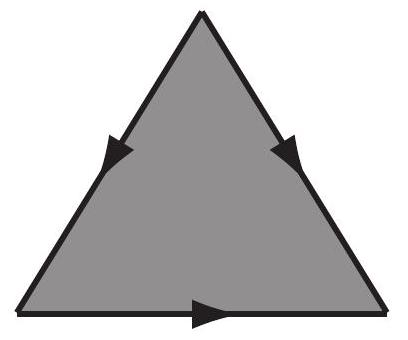
\includegraphics[width=5cm]{sheet 4 q 1 a}\end{center}

\part%1b
Show that the following subspace of $\mathbb{R}^{2}$ cannot be triangulated: \[
	\{(x, y): 0 \leq y \leq 1, \text{ and } x=0 \text{ or } 1 / n, \text { for some } n \in \mathbb{N}\} \cup([0,1] \times\{0\})
\] [\emph{Hint: It is helpful to show that, for any finite simplicial complex $K$, any point $x \in|K|$ and any open set $U$ containing $x$, there is a connected open set $V$ such that $x \in V \subseteq U$.}]
\end{parts}



\question%2
Let $K$ be a simplicial complex (that need not be finite). Prove that $|K|$ is Hausdorff. [\emph{Hint: Recall that a subset of $|K|$ is open if it intersects every simplex in an open set. Note also that the standard simplex has a natural metric as a subset of $\mathbb{R}^{n}$.}]



\question%3
Find an example of a connected, finite, simplicial complex $K$ that is not a closed combinatorial surface, but that satisfies the following three conditions:
\begin{parts}
\part%3a
It contains only 0-simplices, 1-simplices and 2-simplices.

\part%3b
Every 1-simplex is a face of precisely two 2-simplices.

\part%3c
Every point of $|K|$ lies in a 2-simplex.
\end{parts}



\question%4
A simple closed curve $C$ in a space $X$ is the image of a continuous injection $S^{1} \to X$. Find simple closed curves $C_{1}$, $C_{2}$, and $C_{3}$ in the Klein bottle $K$ such that
\begin{parts}
\part%4a
$K \setminus C_{1}$ has one component, which is homeomorphic to an open annulus $S^{1} \times(0,1)$.

\part%4b
$K \setminus C_{2}$ has one component, which is homeomorphic to an open Möbius band. [\emph{An open Möbius band is the space obtained from $[0,1] \times(0,1)$ by identifying $(0, y)$ with $(1,1-y)$ for each $y \in(0,1)$.}]

\part%4c
$K \setminus C_{3}$ has two components, each of which is homeomorphic to an open Möbius band.
\end{parts}



\question%5
The following polygon with side identifications is homeomorphic to which surface?
\begin{center}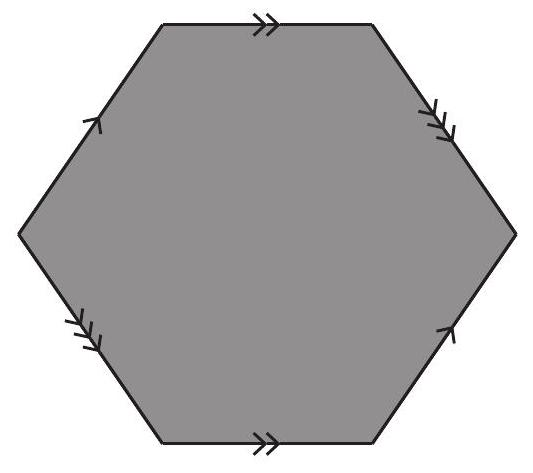
\includegraphics[width=5cm]{sheet 4 q 5}\end{center}



\question%6
Suppose that the sphere $\mathbb{S}^{2}$ is given the structure of a closed combinatorial surface. Let $C$ be a subcomplex that is a simplicial circle. Suppose that $\mathbb{S}^{2} \setminus C$ has two components. Indeed, suppose that this is true for every simplicial circle in $\mathbb{S}^{2}$. Let $E$ be one of these components. [\emph{In fact, $\mathbb{S}^{2} \setminus C$ \emph{must} have 2 components, but we will not attempt to prove this.}]\\ Our aim is to show that $\bar{E}$ is homeomorphic to a disc. This is a version of the Jordan curve theorem. [\emph{The actual Jordan curve theorem is rather stronger than this. It deals with simple closed curves $C$ in $\mathbb{S}^{2}$, which need to be simplicial. It states that $\mathbb{S}^{2} \setminus C$ has two components, and that, for each component $E$ of $\mathbb{S}^{2} \setminus C$, the closure of $E$ is homeomorphic to $\mathbb{D}^{2}$, with the homeomorphism taking $C$ to $\partial \mathbb{D}^{2}$.}]\\ We'll prove this by induction on the number of 2-simplices in $\bar{E}$. Our actual inductive hypothesis is: \emph{There is a homeomorphism from $\bar{E}$ to $\mathbb{D}^{2}$, which takes $C$ to the boundary circle $\partial \mathbb{D}^{2}$.}
\begin{parts}
\part%6a
Let $\sigma_{1}$ be a 1 -simplex in $C$. Since $\mathbb{S}^{2}$ is a closed combinatorial surface, $\sigma_{1}$ is adjacent to two 2-simplices. Show that precisely one of these 2-simplices lies in $\bar{E}$. Call this 2-simplex $\sigma_{2}$.

\part%6b
Start the induction by showing that if $\bar{E}$ contains at most one 2-simplex, then $\bar{E}=\sigma_{2}$.

\part%6c
Let $v$ be the vertex of $\sigma_{2}$ not lying in $\sigma_{1}$. Let's suppose that $v$ does not lie in $C$. Show how to construct a subcomplex $C'$ of $\mathbb{S}^{2}$, that is a simplicial circle, and that has the following properties: \begin{itemize}
  \item $\mathbb{S}^{2} \setminus C'$ has two components;
  \item one of these components $F$ is a subset of $E$;
  \item $\bar{F}$ contains fewer 2-simplices than $\bar{E}$.
\end{itemize} Show in this case that there is a homeomorphism from $\bar{E}$ to $\mathbb{D}^{2}$, which takes $C$ to the boundary circle $\partial \mathbb{D}^{2}$.

\part%6d
Suppose now that $v$ lies in $C$. How do we complete the proof in this case?
\end{parts}

\end{questions}

\end{document}
